% This is the default LaTeX template (default-1.17.0.2.tex) from the RMarkdown package, from:
% https://github.com/rstudio/rmarkdown/blob/master/inst/rmd/latex/default-1.17.0.2.tex
%
% New additions to the template are marked with "LCR"

%\documentclass[12pt,american,]{memoir} %LCR
 % if not, force the oneside and a4paper options, which seem to be the only reasonable defaults
\documentclass[12pt,american,a4paper,oneside,]{memoir} %LCR

\usepackage{lmodern}
\usepackage{amssymb,amsmath}
\usepackage{ifxetex,ifluatex}
\usepackage{fixltx2e} % provides \textsubscript
\ifnum 0\ifxetex 1\fi\ifluatex 1\fi=0 % if pdftex
  \usepackage[T1]{fontenc}
  \usepackage[utf8]{inputenc}
\else % if luatex or xelatex
  \ifxetex
    \usepackage{mathspec}
  \else
    \usepackage{fontspec}
  \fi
  \defaultfontfeatures{Ligatures=TeX,Scale=MatchLowercase}
\fi
% use upquote if available, for straight quotes in verbatim environments
\IfFileExists{upquote.sty}{\usepackage{upquote}}{}
% use microtype if available
\IfFileExists{microtype.sty}{%
\usepackage{microtype}
\UseMicrotypeSet[protrusion]{basicmath} % disable protrusion for tt fonts
}{}

 %LCR
\usepackage{hyperref}
\hypersetup{unicode=true,
            pdftitle={Learning from the brain},
            pdfauthor={Lukas Snoek},
            pdfborder={0 0 0},
            breaklinks=true}
\urlstyle{same}  % don't use monospace font for urls
\ifnum 0\ifxetex 1\fi\ifluatex 1\fi=0 % if pdftex
  \usepackage[shorthands=off,main=american]{babel}
\else
  \usepackage{polyglossia}
  \setmainlanguage[variant=american]{english}
\fi
\usepackage[style=apa]{biblatex}

\addbibresource{thesis.bib}
\usepackage{longtable,booktabs}
% Make links footnotes instead of hotlinks:
\renewcommand{\href}[2]{#2\footnote{\url{#1}}}
\IfFileExists{parskip.sty}{%
\usepackage{parskip}
}{% else
\setlength{\parindent}{0pt}
\setlength{\parskip}{6pt plus 2pt minus 1pt}
}
\setlength{\emergencystretch}{3em}  % prevent overfull lines
\providecommand{\tightlist}{%
  \setlength{\itemsep}{0pt}\setlength{\parskip}{0pt}}
\setcounter{secnumdepth}{5}
% Redefines (sub)paragraphs to behave more like sections
\ifx\paragraph\undefined\else
\let\oldparagraph\paragraph
\renewcommand{\paragraph}[1]{\oldparagraph{#1}\mbox{}}
\fi
\ifx\subparagraph\undefined\else
\let\oldsubparagraph\subparagraph
\renewcommand{\subparagraph}[1]{\oldsubparagraph{#1}\mbox{}}
\fi

%%% Use protect on footnotes to avoid problems with footnotes in titles
\let\rmarkdownfootnote\footnote%
\def\footnote{\protect\rmarkdownfootnote}

%%% This fixes a TexLive 2019 change that broke pandoc template. Will also be fixed in pandoc 2.8 %LCR
% https://github.com/jgm/pandoc/issues/5801
\renewcommand{\linethickness}{0.05em}

\usepackage{caption}
\usepackage[pass]{geometry} % load the package, but none of the default settings
\usepackage{pdflscape} % landscape pages and rotation
\usepackage{bookmark} % section links in pdf
\usepackage{enumitem} % formatting lists
\usepackage[dvipsnames]{xcolor} % prevent error in pdfpages
\usepackage{pdfpages} % for adding the book cover

\let\oldhref\href % save command before redefininig, so we can turn it off again
\renewcommand{\href}[2]{#2\footnote{\url{#1}}} % same as "link-as-notes: true"

\newcommand{\blandscape}{\begin{landscape}}
\newcommand{\elandscape}{\end{landscape}}
\AtBeginDocument{\let\maketitle\relax} % don't make automatic title page as first page

\newcommand{\CoverName}{cover} % to set page numbers of cover pages to "cover"

% change toc depth (to remove subsections in Dutch Summary from toc)
\newcommand{\changelocaltocdepth}[1]{%
  \addtocontents{toc}{\protect\setcounter{tocdepth}{#1}}%
  \setcounter{tocdepth}{#1}%
}

% From https://tex.stackexchange.com/questions/32547/how-to-measure-the-width-of-a-longtable-dynamically-and-use-this-width-in-footer
% papaja requires the \getlongtablewidth command when using the longtable=TRUE option with apa_table
\makeatletter
\newcommand\LastLTentrywidth{1em}
\newlength\longtablewidth
\setlength{\longtablewidth}{1in}
\newcommand{\getlongtablewidth}{\begingroup \ifcsname LT@\roman{LT@tables}\endcsname \global\longtablewidth=0pt \renewcommand{\LT@entry}[2]{\global\advance\longtablewidth by ##2\relax\gdef\LastLTentrywidth{##2}}\@nameuse{LT@\roman{LT@tables}} \fi \endgroup}
\makeatother

%% Typefaces
\usepackage{fontspec}
\setmainfont{Minion Pro}
\setsansfont[Ligatures=TeX]{Helvetica}
\setmathsfont(Digits,Greek,Latin)[Numbers={Proportional}]{Minion Pro}
\setmathrm{Minion Pro}

%% Page layout

% The length of the lowercase alphabet in 11 pt Minion Pro is 127.80293pt (116.7151 pt for 10pt).
% According to equation 2.1 of the memoir manual, the optimal width of the typeblock (66 characters) would then be 294.38358306 pt, or 103.9 mm
% According to table 2.2 of the memoir manual, the typeblock should be between 22 pica's (= 93.13 mm), which would be 59 characters wide, or 26 pica's a little bit more than 22 pica's (= 110.1 mm), which would be 70 characters wide. 

\setstocksize{240mm}{170mm} % adjusted B5, with no bleed on each side for now
\settrimmedsize{240mm}{170mm}{*} % adjusted B5 (standard thesis size)
\setpageml{\paperheight}{\paperwidth}{*} % center the adjusted B5 page to the middle left (so the right, bottom and top will be trimmed)
\settypeblocksize{*}{105mm}{1.618} % typeblock of 105 mm wide (little wider than optimal, to save paper). The golden ratio is a good rule to set the height, which amounts to about 105*1.618 = 170. The actual height of the text block will differ slightly, because it has to fit an integer number of lines.
\setlrmargins{*}{40mm}{*} % leaves 170-105 = 65 mm for margins. Set the foredge margin so its relation to the spine margin is about the golden ratio as well (65/1.618 is 40.2). A foreedge of twice the spine is also common, but I think this makes the foreedge a bit too big. The spine is then 65-40 = 25 mm.
\setulmargins{25mm}{*}{*} % the top margin is often 1/9 of the page height, or 1/9 * 240 mm = 27 mm. Often the top margin is also the same as the spine. Both of these rules almost converge here. 
% This automatically determines the bottom margin at 240 - 25 - 170 = 45. This is bigger than the top margin, which is good, as this is where you hold the book (often the bottom margin is even twice as big as the top).
%\setheadfoot{\onelineskip}{2\onelineskip} % defaults from memoir manual
%\setheaderspaces{*}{2\onelineskip}{*} % defaults from memoir manual
\setmarginnotes{5mm}{15mm}{\onelineskip} % too narrow (15mm, with 5 mm separation from text) for actual margin notes; but some chapter / pagestyles (e.g. companion) run off the page if this is not set.
\settypeoutlayoutunit{mm} % use mm for printing to the log
\checkandfixthelayout

%% Page and chapter styles
\chapterstyle{companion}

\def\defstyle{Ruled} % pagestyle set here will be used on all pages with regular text
\makeevenhead{Ruled}{\leftmark}{}{} % get rid of small caps in verso headers

% distinguish lower-level headings
\setsubsubsecheadstyle{\normalsize\bfseries\itshape} % bold italic
\setparaheadstyle{\normalsize\itshape} % just italic

%% Spacing
\midsloppy % middle ground between overfull lines ("fussy"), or lots of variation in interword spaces ("sloppy")

% try to avoid widows (last line of paragraph at the top of otherwise empty page)
\setlength{\topskip}{1.6\topskip}
\checkandfixthelayout
\sloppybottom

\renewcommand{\arraystretch}{1.5} % increase vertical spacing in tables

% when figures/tables are wider than text block, center them with respect to text block
\setfloatadjustment{figure}{\centerfloat}
\setfloatadjustment{table}{\centerfloat}

%\setlength{\cftpartnumwidth}{2.5em} % more space for part numbering in ToC
%\setlength\cftchapternumwidth{2.5em} % also adjust others to match
%\setlength\cftsectionindent{2.5em} % also adjust others to match

%% Abstracts
\abstractrunin % set "ABSTRACT" title in-line
\renewcommand{\abstractnamefont}{\normalfont\normalsize\scshape\bfseries} % set "ABSTRACT" in bold small scaps
\renewcommand{\abstracttextfont}{\normalfont\normalsize} % normalsize for text
\setlength{\absleftindent}{0pt} % don't increase left margin for abstracts
\setlength{\absrightindent}{0pt} % don't increase right margin for abstracts
\abslabeldelim{\quad} % some space after "ABSTRACT"
% see front_matter.tex for two more commands

%% Part titles 
%format similarly to companion chapter style
\renewcommand{\partnamefont}{\normalfont\huge\scshape}
\renewcommand{\partnumfont}{\normalfont\HUGE}

%\setlength\beforechapskip{-\baselineskip} % this would remove any space above the chapter titles

%% Captions
% Memoir:
%\captionnamefont{\small\sffamily}
%\captiontitlefont{\small\sffamily}
%\hangcaption
% caption package:
\captionsetup{labelfont={rm,sc},textfont={small,sf},labelsep=space} % small sans for table captions, with small caps for label

%% Bibliography
\renewcommand*{\bibfont}{\footnotesize}

% Hyperlink entire author-year citation; not just year
%https://tex.stackexchange.com/questions/15951/hyperlink-name-with-biblatex-authoryear-biblatex-1-4b
\DeclareFieldFormat{citehyperref}{%
  \DeclareFieldAlias{bibhyperref}{noformat}% Avoid nested links
  \bibhyperref{#1}}
\DeclareFieldFormat{textcitehyperref}{%
  \DeclareFieldAlias{bibhyperref}{noformat}% Avoid nested links
  \bibhyperref{%
    #1%
    \ifbool{cbx:parens}
      {\bibcloseparen\global\boolfalse{cbx:parens}}
      {}}}
\savebibmacro{cite}
\savebibmacro{textcite}
\renewbibmacro*{cite}{%
  \printtext[citehyperref]{%
    \restorebibmacro{cite}%
    \usebibmacro{cite}}}
\renewbibmacro*{textcite}{%
  \ifboolexpr{
    ( not test {\iffieldundef{prenote}} and
      test {\ifnumequal{\value{citecount}}{1}} )
    or
    ( not test {\iffieldundef{postnote}} and
      test {\ifnumequal{\value{citecount}}{\value{citetotal}}} )
  }
    {\DeclareFieldAlias{textcitehyperref}{noformat}}
    {}%
  \printtext[textcitehyperref]{%
    \restorebibmacro{textcite}%
    \usebibmacro{textcite}}}

% Handle prefixes in surnames (e.g. "van", "de") correctly
%https://tex.stackexchange.com/questions/440133/prefixes-in-author-names-in-references-and-bibliography
\DeclareSortingNamekeyTemplate{
  \keypart{
    \namepart{family}
  }
  \keypart{
    \namepart{prefix}
  }
  \keypart{
    \namepart{given}
  }
  \keypart{
    \namepart{suffix}
  }
}

\renewbibmacro{begentry}{\midsentence}

%%%%%%%%%%%%% BEGIN DOCUMENT %%%%%%%%%%%%%
\begin{document}

%% Page I: the half-title / "Franse pagina" %LCR
\frontmatter
\thispagestyle{empty}
\def\drop{.1\textheight}

\vspace*{\drop}
\begin{center}
\Huge \textsc{Learning from the brain}
\end{center}

%% Page II: Colophon %LCR
\clearpage
\thispagestyle{empty}
\vspace*{\fill}
\begingroup % to change formatting only temporarily
\small
\setlength{\parskip}{\baselineskip} % add space between paragraphs
\setlength\parindent{0pt} % no indents

This thesis was typeset using (R) Markdown, \LaTeX\ and the \verb+bookdown+ R-package
\\ ISBN: xxx-xx-xxxx-xxx-x\\ Printing: Acme Press, Inc.

An online version of this thesis is available at \url{https://lukas-snoek.com/thesis}, licensed under a CC BY.
\endgroup

%% Page III: `Title page' mandated by University of Amsterdam %LCR
\clearpage
\thispagestyle{empty}
\vspace*{\drop}
\begin{center}
\Huge\textbf{Learning from the brain}\par
\vspace{\baselineskip}
\Large\textit{Best practices for the use of neuroimaging data\\
in psychology research}\par
\vfill % this space will be whatever is left on the page
\large \textsc{Academisch Proefschrift}\par
\vspace{\baselineskip}
\linespread{1.3}{\normalsize ter verkrijging van de graad van doctor\\
aan de Universiteit van Amsterdam\\
op gezag van de Rector Magnificus\\
prof. dr. ir. K.I.J. Maex\\ % make sure this is the current rector magnificus
\mbox{ten overstaan van een door het College voor Promoties ingestelde commissie,}\\
in het openbaar te verdedigen in de Agnietenkapel\\
op maandag 21 oktober 2021, te 14 uur \\ }\par %
\vspace{\baselineskip}
{\large door}\par
\vspace{\baselineskip}
{\Large Lukas Snoek}\par
\vspace{\baselineskip}
{\large geboren te Hoevelaken}
\end{center}

%% Page IV: info on thesis committee %LCR
\clearpage
\thispagestyle{empty}
\noindent\textbf{Promotiecommissie:}\\
\\
\noindent\begin{tabular}{@{}lll}

Promotor:
&  dr. H.S. Scholte & Universiteit van Amsterdam\\

Copromotor:
&  dr. S. Oosterwijk & Universiteit van Amsterdam\\

\\
Overige leden:
&  prof. dr. R.E. Jack & University of Glasgow\\
&  prof. dr. R.W. Goebel & Maastricht University\\
&  prof. dr. B.U. Forstmann & Universiteit van Amsterdam\\
&  prof. dr. A.H. Fischer & Universiteit van Amsterdam\\
&  prof. dr. D. Borsboom & Universiteit van Amsterdam\\
&  prof. dr. A.G. Sanfey & Radboud University\\
\end{tabular}\\

\noindent Faculteit: Faculteit der Maatschappij- en Gedragswetenschappen

%%%%%%%%%%%%%%%%%%


%Based on template from the "IILC Dissertation Style"
% https://www.illc.uva.nl/PhDProgramme/current-candidates/other/illcdiss.html#latex

% for some reason this cannot be in the preamble
\setlength{\abstitleskip}{-\absparindent}

% Include the cover page
\pagestyle{empty}
\renewcommand{\thepage}{\CoverName} % make sure this page is "numbered" with a name, not as page 1 or I
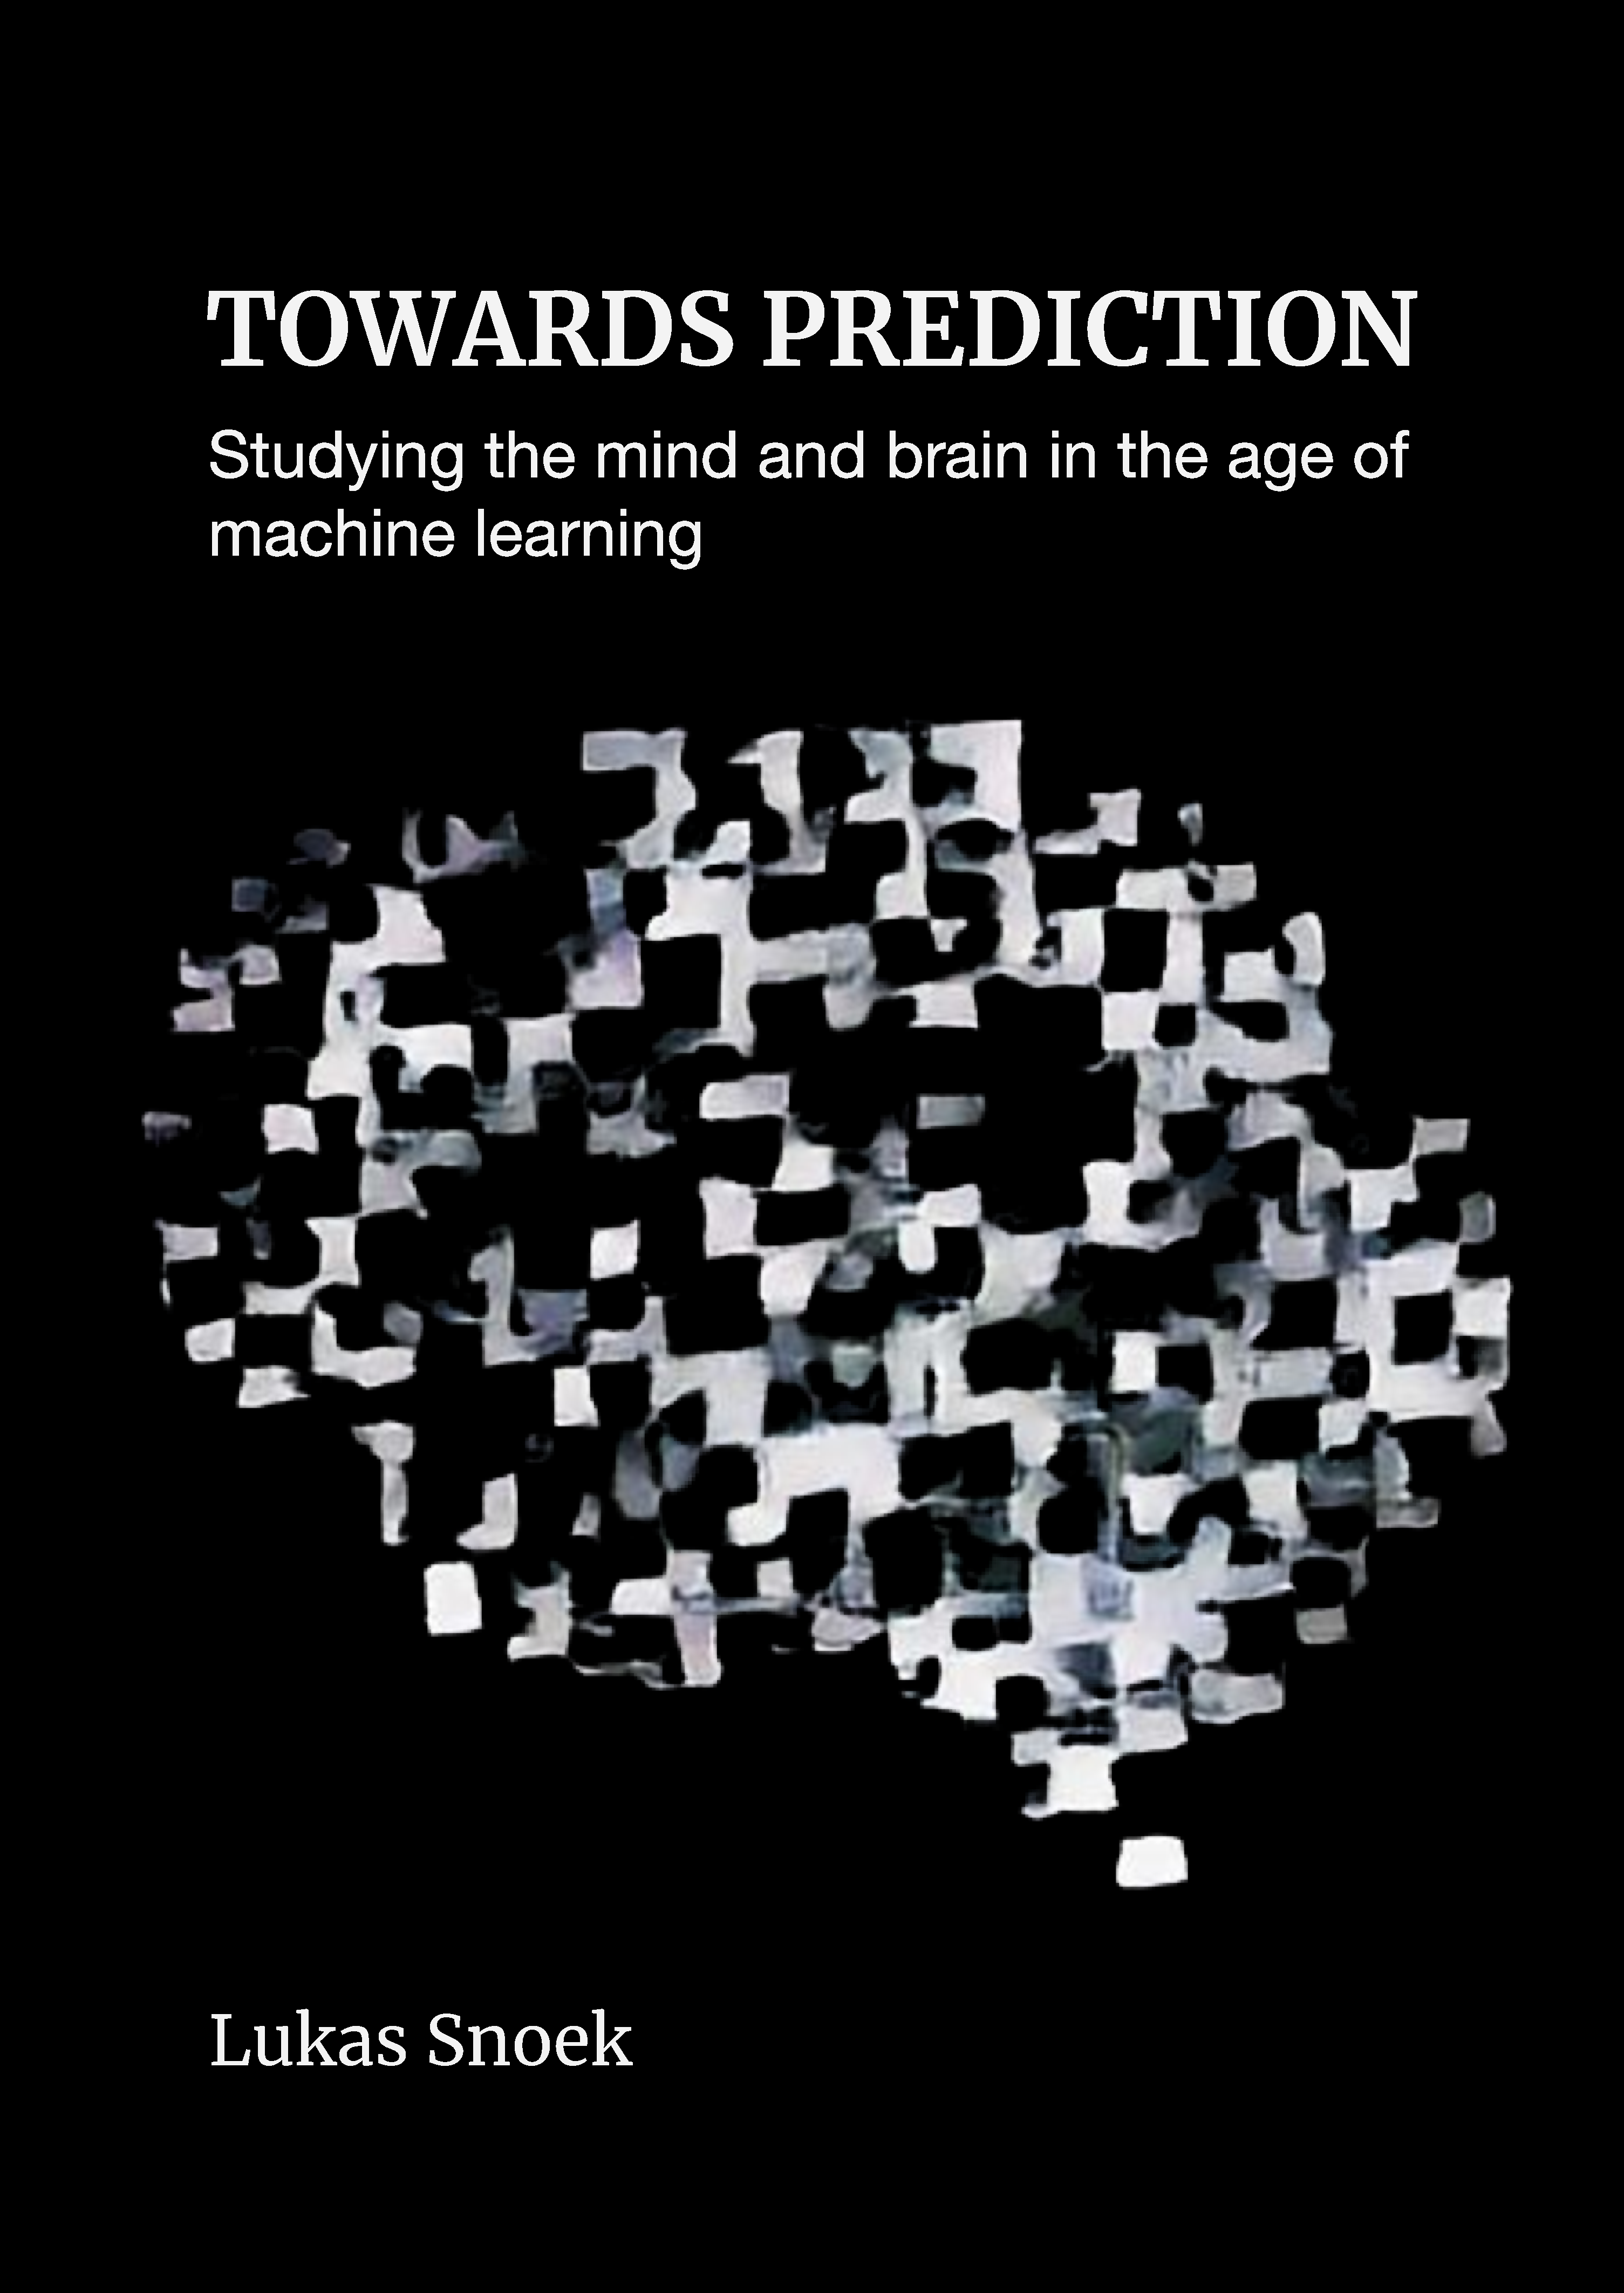
\includepdf{./cover/thesis_cover.pdf}

% \newlength{\mylen}                % a length
% \newcommand{\alphabet}{abcdefghijklmnopqrstuvwxyz} % the lowercase alphabet
% \begingroup                       % keep font change local% font specification e.g., \Large\sffamily
% \settowidth{\mylen}{\alphabet}
% The length of this alphabet is \the\mylen. % print in document\typeout{The length of the Large sans alphabetis \the\mylen}                    % put in log file
% \endgroup                         % end the grouping

{
\setcounter{tocdepth}{1}
\tableofcontents
}
\mainmatter
\hypertarget{introduction}{%
\chapter{Introduction}\label{introduction}}

\emph{The first chapter of the thesis, which introduces your PhD project. The filler-text below was created with the \href{http://www.elsewhere.org/journal/pomo}{postmodernism generator}.}

\begin{center}\rule{0.5\linewidth}{0.5pt}\end{center}

\hypertarget{learning-from-the-brain}{%
\section{Learning from the brain}\label{learning-from-the-brain}}

When reading this thesis' title, some might think that it contains a typo. Scientists want to learn \emph{about} the brain, right? Not \emph{from} the brain. Well, yes, neuroscientists do. But I am a psychologist at heart, interested in human behavior, cognition, and above all, emotion. I'm interested in the mind, not the brain. I don't care about axons, neurotransmitters, and the basal ganglia. Sure, I do believe, like any proper scientist, that everything we feel, perceive, and do is instantiated in the brain, but I do not necessarily think that \emph{just} studying the brain in isolation is going to teach us anything useful about the human psyche. Mind you, in this PhD you'll find several studies that analyze \emph{brain} data, but realize that my ultimate goal has always been to understand the mind.

\hypertarget{shared-states-using-mvpa-to-test-neural-overlap-between-self-focused-emotion-imagery-and-other-focused-emotion-understanding}{%
\chapter{Shared states: using MVPA to test neural overlap between self-focused emotion imagery and other-focused emotion understanding}\label{shared-states-using-mvpa-to-test-neural-overlap-between-self-focused-emotion-imagery-and-other-focused-emotion-understanding}}

\chaptermark{Shared states}

\vspace*{\fill}

\begin{center}\rule{0.5\linewidth}{0.5pt}\end{center}

\small

\noindent
\emph{This chapter has been published as}: Oosterwijk, S.*, Snoek, L.*, Rotteveel, M., Barrett, L. F., \& Scholte, H. S. (2017). Shared states: using MVPA to test neural overlap between self-focused emotion imagery and other-focused emotion understanding. \emph{Social cognitive and affective neuroscience, 12}(7), 1025-1035.

* Shared first authorship
\newpage
\normalsize

\textbf{Abstract}

The present study tested whether the neural patterns that support imagining ``performing an action'', ``feeling a bodily sensation'' or ``being in a situation'' are directly involved in understanding \emph{other people's} actions, bodily sensations and situations. Subjects imagined the content of short sentences describing emotional actions, interoceptive sensations and situations (self-focused task), and processed scenes and focused on \emph{how} the target person was expressing an emotion, \emph{what} this person was feeling, and \emph{why} this person was feeling an emotion (other-focused task). Using a linear support vector machine classifier on brain-wide multi-voxel patterns, we accurately decoded each individual class in the self-focused task. When generalizing the classifier from the self-focused task to the other-focused task, we also accurately decoded whether subjects focused on the emotional actions, interoceptive sensations and situations of \emph{others}. These results show that the neural patterns that underlie self-imagined experience are involved in understanding the experience of other people. This supports the theoretical assumption that the basic components of emotion experience and understanding share resources in the brain.

\hypertarget{Sharedstates-introduction}{%
\section{Introduction}\label{Sharedstates-introduction}}

To navigate the social world successfully it is crucial to understand other people. But how do people generate meaningful representations of other people's actions, sensations, thoughts and emotions? The dominant view assumes that representations of other people's experiences are supported by the same neural systems as those that are involved in generating experience in the self \autocites[e.g.,][]{gallese2004unifying}[see for an overview][]{singer2012past}. We tested this principle of self-other neural overlap directly, using multi-voxel pattern analysis (MVPA), across three different aspects of experience that are central to emotions: actions, sensations from the body and situational knowledge.

In recent years, evidence has accumulated that suggests a similarity between the neural patterns representing the self and others. For example, a great variety of studies have shown that observing actions and sensations in other people engages similar neural circuits as acting and feeling in the self \autocite[see for an overview][]{bastiaansen2009evidence}. Moreover, an extensive research program on pain has demonstrated an overlap between the experience of physical pain and the observation of pain in other people, utilizing both neuroimaging techniques \autocite[e.g.,][]{lamm2011meta} and analgesic interventions \autocites[e.g.,][]{rutgen2015placebo}{mischkowski2016painkiller}. This process of ``vicarious experience'' or ``simulation'' is viewed as an important component of empathy \autocite{carr2003neural,decety2011dissecting,keysers2014dissociating}. In addition, it is argued that mentalizing (e.g.~understanding the mental states of other people) involves the same brain networks as those involved in self-generated thoughts \autocite{uddin2007self,waytz2011two}. Specifying this idea further, a constructionist view on emotion proposes that both emotion experience and interpersonal emotion understanding are produced by the same large-scale distributed brain networks that support the processing of sensorimotor, interoceptive and situationally relevant information \autocite{barrett2013large,oosterwijk2014embodiment}. An implication of these views is that the representation of self- and other-focused emotional actions, interoceptive sensations and situations overlap in the brain.

\hypertarget{how-to-control-for-confounds-in-decoding-analyses-of-neuroimaging-data}{%
\chapter{How to control for confounds in decoding analyses of neuroimaging data}\label{how-to-control-for-confounds-in-decoding-analyses-of-neuroimaging-data}}

\hypertarget{the-amsterdam-open-mri-collection-a-set-of-multimodal-mri-datasets-for-individual-difference-analyses}{%
\chapter{The Amsterdam Open MRI Collection, a set of multimodal MRI datasets for individual difference analyses}\label{the-amsterdam-open-mri-collection-a-set-of-multimodal-mri-datasets-for-individual-difference-analyses}}

\hypertarget{choosing-to-view-morbid-information-involves-reward-circuitry}{%
\chapter{Choosing to view morbid information involves reward circuitry}\label{choosing-to-view-morbid-information-involves-reward-circuitry}}

\hypertarget{using-predictive-modeling-to-quantify-the-importance-and-limitations-of-action-units-in-emotion-perception}{%
\chapter{Using predictive modeling to quantify the importance and limitations of action units in emotion perception}\label{using-predictive-modeling-to-quantify-the-importance-and-limitations-of-action-units-in-emotion-perception}}

\hypertarget{comparing-models-of-dynamic-facial-expression-perception}{%
\chapter{Comparing models of dynamic facial expression perception}\label{comparing-models-of-dynamic-facial-expression-perception}}

\backmatter

\hypertarget{bibliography}{%
\chapter*{Bibliography}\label{bibliography}}
\addcontentsline{toc}{chapter}{Bibliography}

\markboth{\MakeUppercase{Bibliography}}{} % have to explicitly state what to put in the heading (bug in bookdown?)
%format the references so they have a hanging indent. Remove these (and the \endgroup command) if you want regular indentation.
\begingroup
\hspace{\parindent}
\setlength{\parindent}{-0.25in}
\setlength{\leftskip}{0.25in}
\setlength{\parskip}{0pt}

\hypertarget{refs}{}

\endgroup

\backmatter
\printbibliography


\end{document}
